\begin{figure}[ht]
    \centering
    \includegraphics[width=1\textwidth]{figures/views/gel-list.png}
    \caption{\textit{Application gel list view.}}
    \label{fig:gel-list}
\end{figure}

\begin{figure}[ht]
    \centering
    \includegraphics[width=1\textwidth]{figures/views/gel-lanes-popup.png}
    \caption{\textit{Application gel lanes popup view.}}
    \label{fig:gel-lanes-popup}
\end{figure}

\begin{figure}[ht]
    \centering
    \includegraphics[width=1\textwidth]{figures/views/types-list.png}
    \caption{\textit{Application measurement types list view.}}
    \label{fig:types-list}
\end{figure}

\begin{figure}[ht]
    \centering
    \includegraphics[width=1\textwidth]{figures/views/gel-detail.png}
    \caption{\textit{Application gel detail view.}}
    \label{fig:gel-detail}
\end{figure}

\begin{figure}[ht]
    \centering
    \includegraphics[width=1\textwidth]{figures/views/image-selection-popup.png}
    \caption{\textit{Application image selection popup view (local folder).}}
    \label{fig:gel-image-selection-popup}
\end{figure}

\begin{figure}[ht]
    \centering
    \includegraphics[width=1\textwidth]{figures/views/gel-image-raw.png}
    \caption{\textit{Application image raw view.}}
    \label{fig:gel-image-raw}
\end{figure}

\begin{figure}[ht]
    \centering
    \includegraphics[width=1\textwidth]{figures/views/gel-image-adjust.png}
    \caption{\textit{Application image adjust view.}}
    \label{fig:gel-image-adjust}
\end{figure}

\begin{figure}[ht]
    \centering
    \includegraphics[width=1\textwidth]{figures/views/gel-image-bg-sub.png}
    \caption{\textit{Application image background subtraction view.}}
    \label{fig:gel-image-bg-sub}
\end{figure}

\begin{figure}[ht]
    \centering
    \includegraphics[width=1\textwidth]{figures/views/gel-image-lanes.png}
    \caption{\textit{Application image lanes view.}}
    \label{fig:gel-image-lanes}
\end{figure}

\begin{figure}[ht]
    \centering
    \includegraphics[width=1\textwidth]{figures/views/gel-image-measurements.png}
    \caption[\textit{Application image measurements view.}]%
    {\textit{Application image measurements view.}}
    {\small {a) lanes graph}, {b) intensity plots}} \\
    {\small {c) measurement lanes table}, {d) measurements table}}
    \label{fig:gel-image-measurements}
\end{figure}

\begin{figure}[ht]
    \centering
    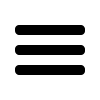
\includegraphics[width=1\textwidth]{figures/views/settings.png}
    \caption{\textit{Application settings view.}}
    \label{fig:settings}
\end{figure}
